\section{Introduction}

Large language model (LLM) decoding is increasingly limited by data movement rather than raw arithmetic throughput, especially as context length grows and KV-cache traffic expands. This has renewed interest in processing-in-memory (PIM) style acceleration for inference. Recent PIM and near-memory systems papers show that decode workloads can expose kernels with different bottleneck types, which suggests that dynamic offloading may matter. However, an important question remains underexplored: \emph{when does virtual PIM offloading actually become worthwhile during decoding, and what signal best predicts regime entry?}

This question is easy to ask but difficult to answer cleanly. Real PIM-enabled heterogeneous systems are expensive to build, production LLM serving stacks hide many low-level details, and performance conclusions are sensitive to workload regime. As a result, it is difficult to separate three issues: whether offload value is real at all, which runtime conditions trigger it, and whether simple heuristics such as ``offload attention'' are sufficient to detect those conditions.

We study this problem using a trace-driven virtual PIM evaluation framework for LLM decoding. Our framework instruments open-source decoding runs, extracts region-level traces and runtime features, and replays them through a prior-work-grounded virtual PIM cost model. This lets us evaluate static and dynamic decision rules on real decode behavior while explicitly avoiding direct hardware-speedup claims. The goal is not to introduce a new PIM architecture, but to characterize the operating regimes in which PIM-style offloading appears useful and the runtime signals that best predict those regimes under a transparent virtual backend.

The central empirical result is a consistent weak-signal versus positive-signal split. Short-context decoding often shows no realistic gain even when an oracle policy still has latent upside, which means the framework is not fabricating benefits everywhere. In contrast, longer-context decoding repeatedly enters a positive offload regime. Dense context sweeps sharpen this transition and show that context length is the clearest coarse regime-entry variable in our current setup, but the onset is model-family dependent. For example, \texttt{Qwen2.5-1.5B} shows delayed onset, while \texttt{Qwen3-8B}, \texttt{SmolLM2-1.7B}, and \texttt{Phi-3.5-mini} enter the positive regime earlier. We further find that KV-cache-related signals are more consistent with the observed boundary than attention labels alone, but we treat this as predictive evidence rather than as a causal proof.

\begin{figure}[t]
    \centering
    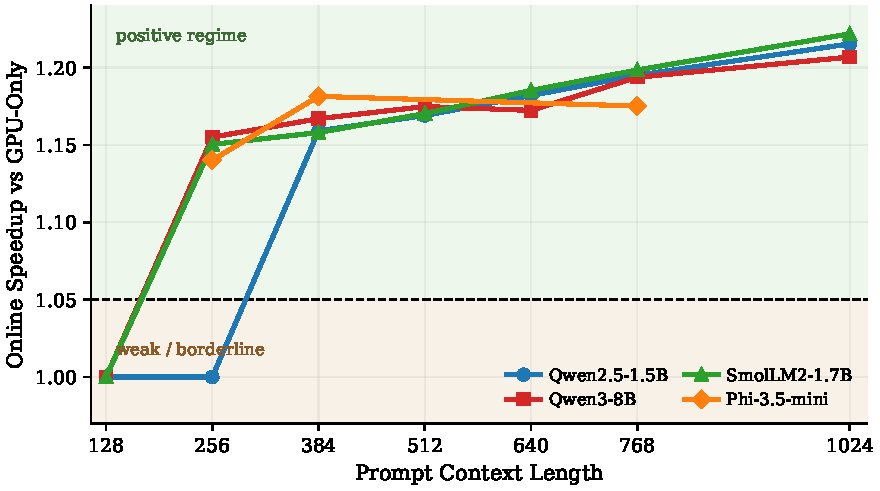
\includegraphics[width=0.95\linewidth]{figures/final_figures/paper_backbone_context_transition.pdf}
    \caption{Dense context sweeps show that virtual PIM benefit is regime-dependent rather than universal. In our current setup, context length is the clearest coarse regime-entry variable, but onset is family-dependent: \texttt{Qwen2.5-1.5B} enters later than \texttt{Qwen3-8B}, \texttt{SmolLM2-1.7B}, and \texttt{Phi-3.5-mini}.}
    \label{fig:context-transition}
\end{figure}

These observations lead to a narrower and safer policy message than ``dynamic scheduling is better.'' A static attention heuristic is directionally useful, but it is too permissive. A generic realistic feature policy is also too conservative in several important cases. In contrast, KV-aware features can help refine boundary detection in some early-positive families, which suggests that the core decision problem is not merely to identify attention regions, but to detect when a decode stream has plausibly crossed into a positive offload regime.

Our contribution is therefore an empirical systems characterization rather than a hardware paper. We do not claim real PIM speedups, cycle-accurate backend fidelity, or a final deployment-ready scheduler. Instead, we make the following contributions:

\begin{itemize}
\item We present a trace-driven framework for studying virtual PIM decision signals during LLM decoding using runtime-grounded traces, a transparent virtual PIM backend, and policy replay.
\item We show that virtual PIM value is regime-dependent: short-context decoding is often weak or borderline, while longer-context decoding repeatedly enters a positive offload regime.
\item We show that context length is the clearest coarse regime-entry variable in our current setup, but that the onset of positive offload value is model-family dependent.
\item We show that the observed boundary is consistent with explicit KV-cache pressure proxies, and that KV-aware features can complement coarse context cues for positive-regime detection.
\end{itemize}

The rest of the paper is organized as follows. \Cref{sec:related} positions this work relative to prior PIM, KV-cache, and scheduling systems. \Cref{sec:method} describes the trace-driven framework and the evaluation protocol. \Cref{sec:experiments} presents the regime characterization, mechanism evidence, and policy analysis. \Cref{sec:conclusion} concludes with limitations and future directions.
